\documentclass[11pt]{standalone}

\usepackage{garamondx}
\usepackage{pgfplots}
\usepackage{tikz}
\usepgfplotslibrary{units}
\usepackage{xcolor}
\definecolor{redtea}{rgb}{0.6823529412,0.2792156863,0.2666666667}
\usepackage{siunitx}
\usepackage{changepage}
\usepackage{calc}
\pgfplotsset{samples}
\usetikzlibrary{arrows,shapes,snakes,automata,backgrounds,petri,positioning}

\pgfdeclarelayer{background}
\pgfdeclarelayer{foreground}
\pgfsetlayers{background,main,foreground}




\begin{document}
	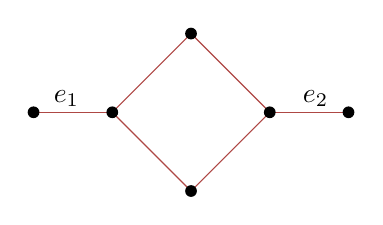
\begin{tikzpicture}
	\coordinate[] (centre) at (0,0);
	\coordinate[] (n1) at (0,1);
	\coordinate[] (n2) at (1,0);
	\coordinate[] (n3) at (0,-1);
	\coordinate[] (n4) at (-1,0);
	\coordinate[] (n5) at (-2,0);
	\coordinate[] (n6) at (2,0);
	
	
	
	\draw[redtea](n1)--(n2);
	\draw[redtea](n2)--(n3);
	\draw[redtea](n3)--(n4);
	\draw[redtea](n4)--(n5);
	\draw[redtea](n4)--(n1);
	\draw[redtea](n2)--(n6);
	
	\node at (centre)[]{};
	\node at (n1)[circle,fill,inner sep=1.5pt]{};
	\node at (n2)[circle,fill,inner sep=1.5pt]{};
	\node at (n3)[circle,fill,inner sep=1.5pt]{};
	\node at (n4)[circle,fill,inner sep=1.5pt]{};
	\node at (n5)[circle,fill,inner sep=1.5pt]{};
	\node at (n6)[circle,fill,inner sep=1.5pt]{};
	
	
	\node[left=of n4,xshift=2em,yshift=0.5em]{$e_1$};
	\node[right=of n2,xshift=-2em,yshift=0.5em]{$e_2$};
	%\draw[->,>=latex,redtea,shorten >=5pt]([xshift=3pt,yshift=0pt]a)--([xshift=3pt,yshift=0pt]b);
	%\draw[->,>=latex,redtea,shorten >=5pt]([xshift=0pt,yshift=0pt]a)--([xshift=0pt,yshift=0pt]a);
	\end{tikzpicture}
\end{document}
